\chapter{Introduction au domaine}

Dans un premier temps, il est important d'évoquer ce qui caractérise les architectures que nous emploierions lors de nos tests ainsi que les méthodes de parallélisation et leurs différences de fonctionnement.

\section{ Les différentes architectures }

Aujourd'hui il existe de nombreuses architectures de processeurs différentes au sein de nos machines aussi bien dans les ordinateurs que dans les appareils nomades. Nous allons explorer deux grandes familles :
les architectures ARM (Advanced RISC Machines) utilisées dans les appareils nomades et les architectures x86 (et x86-64) utilisées dans la plupart des ordinateurs.

\subsection{ Les architectures Advanced RISC Machines (ARM)}

Les architectures ARM sont introduites en 1983 mais elle ne s'insère que depuis quelques années sur le marché des appareils nomades. elles sont basés sur des architectures RISC (Reduced Instruction Set Computer) 32 bits (ARMv3 à ARMv7) et récemment 64 bits avec l'ARMv8. Aujourd'hui, le développement autour de cette architecture a atteint son apogée. On assiste à une augmentation des fréquences constante ainsi qu'au nombre de cœurs qu'un processeur possède.

\subsubsection{ Reduced Instruction Set Computer }

Comme introduit précédemment, l'architecture employée pour l'ARM est RISC. il s'agit d'un type d'architecture matérielle de microprocesseur. Elle est caractérisée par un jeu d'instructions réduit, facile à décoder et comportant uniquement des instructions simples. Elle s'oppose à l'architecture CISC (Complex Instruction Set Computer) employé sur les architectures x86 et x86-64 que nous décrirons plus tard.
\\
Ce type d'architecture est caractérisée par le fait de reposer l'optimisation du code sur le compilateur tandis que les instructions sont faciles à décoder pour le processeur. Pour cela :
\begin{itemize}
\item Ces processeurs possèdent un nombre important de registres "généraux" (un minimum de 16 et généralement de 32). Ils sont tous équivalents afin de faciliter leur allocation par le compilateur
\item Les instructions possèdent une taille fixe, souvent de 32 bits
\item Les instructions utilisées pour des calculs arithmétiques possèdent généralement 3 adresses avec 2 registres comme opérandes et un registre de sortie
\item Pour les accès à la mémoire, des instructions spécifiques sont employées et une valeur doit, au préalable, être chargée dans un registre pour être utilisée. Ce genre d'architecture est nommé load-store ou instruction register-register
\end{itemize}
Afin d'en améliorer les performances, des ajouts ont été effectuées. Par exemple des instructions plus petites ou des méthodes de compression de code ont été ajoutés ou encore les fenêtres de registres qui permettent une accélération des appels de fonctions sur certaines architectures.
Les architectures actuelles ont aussi la possibilité d'utiliser des instructions vectorielles et une unité de calcul en virgule flottante. 
\\
Ce type d'architecture possèdent plusieurs avantages dont l'un d'eux consiste principaux à la présence d'instructions simples. En effet, grâce à ce type d'instruction, l'exécution du processeur est rapide, idéalement en un seul cycle, voire deux instructions en un cycle. Par exemple, certains processeurs RISC présents sur des calculateurs plus puissants se sont vu ajouter des instructions du type MULADD (multiplication + addition). Ce type d'instruction est très utilisé pour des calculs vectoriels et matriciels. Cela avait pour effet, par exemple, de prendre un seul cycle pour multiplier deux registres, y ajouter un autre registre et sauvegarder le résultat dans l'un de ces registres ou dans un autre.\\
Un autre avantage consiste à la faible perdition thermique de ce type de processeur contrairement au architecture CISC. En effet, on constate une utilisation des processeurs ARM sur des appareils mobiles sans un système de refroidissement lourd (ventilateur) contrairement aux ordinateurs équipé d'un processeur CISC.
\\
Mais ce type d'architecture n'est pas sans inconvénient dont l'un correspond à la faible lisibilité du code d'un programme en assembleur surtout lorsqu'une optimisation de celui-ci est nécessaire.
un autre inconvénient est le fait que son code est généralement moins compact car toutes les instructions sont de même taille au contraire des instructions CISC qui sont généralement plus courtes.  

\subsubsection{ SoC (System on Chip) }

Quand on évoque les processeurs ARM, on parle aussi d'un System on Chip ou SoC car ceux-ci sont rarement employés seuls. Il s'agit d'une puce intégrant un microprocesseur, un processeur graphique, d'autres fonctionnalité et contrôleur de périphériques. Ce type de système se retrouve majoritairement sur les tablettes et les smartphones. L'ARM propose des architectures différentes selon le SoC employé. Chacun des constructeurs exploitant l'ARM peut ainsi ajouter des options propres ou de concepteurs tiers à leur architecture. Ainsi on a vu apparaitre, pour les socles d'aujourd'hui, les microprocesseurs Cortex, l'Apple A6 par exemple composé de technologie du cortex-A9 et cortex-A15 ou encore le TEGRA produit par Nvidia ayant une orientation plus vers la capacité graphique.

\begin{figure}[h!]
\begin{center}
	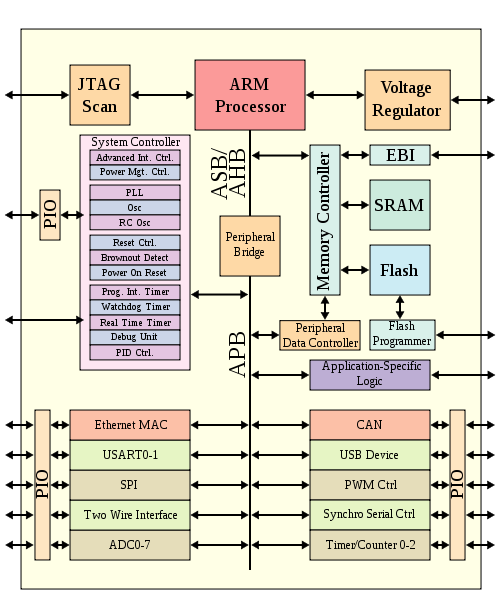
\includegraphics[scale=0.9]{ARMSoCBlockDiagram.png}
	\caption{Exemple de SoC}
\end{center}
\end{figure}

\clearpage

\subsection{ Les architectures x86 et x86-64 }

L'architecture x86(32 bits) ou x86-64(64 bits) sont les architectures les plus utilisées sur les ordinateurs aujourd'hui. Elles utilises les jeux d'instructions du type CISC (Complex instruction set computer). Ce type d'architecture comporte aussi des processeurs multicœurs mais aussi des processeurs utilisant l'hyper-threading que nous détaillerons dans les parties suivantes.

\subsubsection{ Complex instruction set computer }

Comme évoquer précédemment, cette architecture de processeur utilise des jeux d'instruction du type CISC utilisant de très nombreuses instructions mixées à des modes d'adressages complexes. \\
Ce type de jeu d'instructions possède plusieurs avantages :
\begin{itemize}
	\item L'empreinte mémoire du code est beaucoup plus dense. Par exemple on observe un facteur deux entre de l'ARM thumb et le x86). Cela pour effet de permettre l'utilisation minimale de la taille du cache instruction.
	\item Elle permet aussi de la microprogrammation, donc de corriger le jeu d'instructions. Cela facilite la correction de bug.
	\item Avec l'architecture CISC, on peut utiliser des instructions plus complexes non ou mal gérer par les compilateurs mais très rapide.
\end{itemize}
Ce type de microprocesseurs est plus difficile à accélérer. Leur structure est généralement plus complexe que sur une architecture RISC.

\subsubsection{ Hyper-threading }

Pour la réalisation de nos tests sur des machines d'architecture x86-64, 
nous rencontrerons l'hyper-threading. Développé par Intel, cela consiste schématiquement à doter un processeur de deux processeurs logiques sur une seule puce ayant, pour chacun, ses propres registres de données et de contrôle ainsi qu'un contrôleur d'interruption particulier. Ces deux unités partagent les éléments du cœur processeur, le bus système et le cache. Grâce à cette technologie, le processeur peut traiter deux sous processus simultanément. Au niveau des performances, cela ne remplace pas ceux d'un vrai cœur mais la présence de l'hyper-threading peut avoir une influence sur les futurs tests et donc sur les comparaisons. 

\section{ Les méthodes de parallélisations }

Dans cette section, nous allons lister plusieurs méthodes ou technologies de parallélisations que nous allons employer lors de nos tests. Il existe certaines méthodes appartenant à un type d'architecture évoquer précédemment comme le SSE (Streaming SIMD Extensions) pour les processeurs x86-64 ou NEON (Advanced SIMD) les processeurs ARM.

\subsection{ Thread }


 




 



